\documentclass[10pt,a4paper]{article}
\usepackage[latin1]{inputenc}
\usepackage{amsmath}
\usepackage{amsfonts}
\usepackage{amssymb}
\usepackage{graphicx}
\usepackage{natbib}
\usepackage[margin=0.75in]{geometry}
\usepackage{setspace}
\begin{document}
\doublespacing


\tableofcontents
\listoffigures
\listoftables

\section{Introduction}
\subsection{Motivation}
	Continental deformation occurs far from plate boundaries. The behavior of intraplate fault systems is poorly understood. Furthermore, complex kinematics can occur at the intersection of multiple fault systems. Understanding how and why these deformation patterns develop is important for understanding broad active tectonic patterns, reconstructing past tectonics, analyzing seismic hazard and identifying potential resources. The Altai Range and the Gobi-Altai Range are two large, actively forming, mountain ranges in central Asia. The Altai Range is characterized by right-lateral transpressional slip, while the Gobi-Altai Range is characterized by left-lateral transpressional slip \citep{Cunningham2005a}\citep{Cunningham2010}. The intersection of these two fault systems provides a natural laboratory for studying strike-slip kinematics in an area with a long, varied tectonic history. Furthermore, an understanding of this critical zone will help elucidate the evolution of regional tectonic patterns.
	
\begin{figure}[h!]
	\centering
	\includegraphics[width = 6.5in, height = 4in]{broad.png}
	\caption{Shaded relief map of Mongolia with fault overlays and seismic moment tensor solutions for recorded earthquakes. Important locations or faults are labeled. The study area and location of Figure \ref{regional} is outlined in black. Modified after \citet{Calais2003}}
	\label{broad}
\end{figure}

\begin{figure}[h!]
	\centering
	\includegraphics[width = 6in, height = 4in]{regional.png}
	\caption{Shaded relief map showing notable features in the Shargyn Basin region. GPS velocity magnitude for the Altai site is 4.4mm/yr. Faults are shown. See Figure \ref{faultmap} for slip.}
	\label{regional}
\end{figure}
	
	The 150km wide Shargyn Basin in western Mongolia lies at the intersection of the Altai fault system and the Gobi-Altai fault system. In this report, I describe the Shargyn Basin as the result of transpressional strike-slip kinematics. The kinematics can be described as a combination of a compressional strike-slip stepover, a conjugate strike-slip intersection and termination thrust splays. I also use geophysical data to argue that a difference in basement rock has been a primary control on the neotectonic development of the Shargyn Basin region.

\subsection{Mongolian Deformation}
For a region so far from a plate margin, the rate of crustal deformation in Mongolia is very high. GPS measurements (Figure \ref{broad}) show that ongoing motion is to the north in the Altai, and mostly eastward in the Gobi-Altai\citep{Calais2003}. The average rate of motion is approximately 5 mm/year. Multiple earthquakes with a moment magnitude of 8 or greater have occured in the last century. In July 1905, earthquakes with mangitude 7.9 and 8.4 occured on the Bolnay Fault in northern Mongolia. The 1957, magnitude ~8.0 earthquake on the Bogd Fault is one of the best exposed strike-slip surface ruptures in the world\citep{Kurushin1998} \citep{Okal1976a} \citep{Pollitz2003}. It has been used as an analogue for potential Southern California earthquake events \citep{Bayarsayhan1996}. These three earthquakes are some of the largest strike-slip earthquakes ever, emphasizing the intensity of intracontinental deformation in Mongolia. The intensity of deformation makes Mongolia an ideal place to study the mechanics of intracontinental fault systems.

	Active deformation in Mongolia is mostly a result of the Indian-Eurasian collision. However, theoretical models of crustal deformation in Eurasia suggest that the deformation rates in Mongolia are too large to be entirely explained by the India-Eurasia collision \citep{Calais2002a}. Also, some of the deformation in Central and Eastern Asia may have begun before the India-Eurasia collision \citep{Schellart2005}. Nonetheless, many of the large scale features of Central and Eastern Asia can be replicated by a rigid impactor (India) hitting a plasticine block (Eurasia) with a free "eastern" surface (the East Asian Subduction Zone)\citep{Tapponnier1982}. Most importantly, this model showed that the collision of India would cause blocks of Eurasia to "extrude" to east, into the East Asian Subduction Zone.  Many of the large-scale features predicted by this model have been confirmed \citep{Schellart2005}\cite{Yin2010}. The far-field effects of this model are a major component of the recent stresses in Mongolia. 

	 Rollback on the East Asian Subduction System (EASS) provides an additional explanation for active and past motions in Mongolia \citep{Schellart2005}. Classically, researchers described the EASS as a free-boundary. But, because of its orientation, active East Asian Subduction System rollback would exert similar stresses to the Indian-Eurasian collision. However, the potential for far-field stresses from subduction zone rollback is not well constrained. Back-arc extension may not be limited to the deep, ocean-floor producing, back-arc basins. It is suggested that much of the East Asian Subduction zone was experiencing rollback during the late Cretaceous until the Mid-Miocene. A physical model by \citet{Schellart2005} showed that, if the entire East Asian Subduction zone were to rollback, intraplate deformation could occur as far as 3000km from the subduction zone. Additional constraints on the active and past deformation in Mongolia could influence this rollback theory. 

\begin{figure}[h!]
	\centering
	\includegraphics[width = 6.6in, height = 6in]{asia.png}
	\caption{"Simplified tectonic map of East Asia and the Western Pacific illustrating latest Cretaceous and Cenozoic faults in East Asia. 1, 2 and 3 are major thrust, strike-slip and normal fault, respectively; 4, 5 and 6 are convergent (filled triangles are for active and open triangles are for inactive boundary), transform and divergent plate boundary, respectively; 7 is land; 8 is sea, with dark grey being basin or ocean floor and light grey being continental shelf or morphological high on basin or ocean floor. BHb, Bohaiwan basin; BSb, Banda Sea basin; CKg, Central Kamchatka graben; ECSb, East China Sea basin; FMg, Fushun-Meikehou graben; Fr, Fenwei rift; HYr, Hetao-Yinchuan rift; Jb, Java basins; MGb, Mergui basin; MLb, Malay basin; OT, Okinawa Trough; Pb, Pattani basin; Sb, Sumatra basins; SCSb, South China Sea basin; SCSmb, South China Sea marginal basin; SHdsz, Sakhalin-Hokkaido dextral shear zone; SLb, Shantar-Liziansky basin; SXr, Shanxi rift; Yb, Yunqing basin; YSb, Yellow Sea basin; YYg, Yilan-Yitong graben; Zb, Zengmu basin; Zu, Zenghe uplift" \citep{Schellart2005}. I have made additions to the figure: The location of Figure \ref{broad} is outlined in Central Asia. Gray arrows are added to indicate the direction of motion. The left-slip shear zone with accompanying right-slip bookshelf faults is surrounded by a dashed line. Note the continued left-slip shear all the way to the Pacific coast.}
\end{figure}

	On the broadest scale, the Altai and Gobi-Altai fault systems may be related to a sequence of regularly-spaced, NW-SE striking right-lateral strike-slip faults \citep{Yin2010} located in a belt from west Mongolia through Iran. Many of these faults terminate in large thrust systems like the Tian Shan. One explanation of these right-lateral faults explain them as accomodating bookshelf-like rotation in a massive 3500km long  to accomodate the left-lateral shear. (CITE DELVAUX) \citep{Bayasgalan2005a} This model implies that the development of the Altai and Gobi-Altai is intimately linked to that of the Tian Shan. Perhaps the Altai and Gobi-Altai represent an earlier phase in the evolution of the Tian Shan, given the progressive northward propagation of stresses as the India-Eurasian collision proceeds.

	Recent studies have examined the neotectonics of the Altai range via satellite imagery and targeted field excursions\citep{Cunningham2005a}. The region is dominated by NW-SE striking right-lateral slip. The primary features are strike-slip faults, but much of the topography is created by thrusts oriented 30 degrees off the main strike slip faults. Some of these thrusts are isolated. Others are linked by a right-slip faults. In some places, the thrusts are part of a restraining bend. Pure strike-slip, oblique slip and thrust earthquake moment tensors are observed, which indicates that active motion is variable depending on the specific fault \citep{Bayasgalan2005a}.  

Southeast of the Altai, deformation in the Gobi-Altai range is predominantly E-W striking left-lateral slip \citep{Cunningham2010}. North and south dipping thrusts striking NW-SE follow the basement structures, whereas the strike-slip faults cut across the basement structures. Most of the topography is formed by restraining bends or isolated thrusts. The deformation is diffuse over a 250-350km north-south extent. The range accomodate the eastwards and northeastwards deformation as measured by GPS. At the southern extent of the range, the Gobi-Tian Shan Fault is continuous from the easternmost Tian Shan through the eastern Gobi-Altai, thus supporting the connection between the Gobi-Altai and the Tian Shan Some estimates suggest 30-40km of Cenozoic slip on the Gobi-Tien Shan Fault System (CITE Cunningham 2003 about Tian Shan). There are no slip estimates for the Bogd Fault System in the north. However, empirical relationships between fault slip and fault length suggest that the Bogd Fault System has experienced at least 10km of slip \citep{Cowie1992}.  Earthquake moment tensors show primarily left-lateral strike-slip in the Gobi-Altai. 

(CLEAN UP THIS PARAGRAPH, it's ugly) Previously, it was thought that the Hangay Dome, a large domal uplift in central western Mongolia, behaved as an indenter causing the formation of a pair of conjugate strike-slip faults (Altai and Gobi-Altai fault systems). However, recent detailed mapping work has shown the presence of large strike-slip structure cutting across the Hangay Dome \citep{Walker2007}. This indicates that the Hangay Dome is being brittly deformed in a similar fashion to the Gobi-Altai to the south.

\subsection{Shargyn Basin}

	The Shargyn basin is located at the intersection of the Altai fault system and the Gobi-Altai fault system. It is approximately 150km in east-west extent and 100km in north-south extent. A small ephemeral lake is located in the center of the basin. Broad, varying, color bands on satellite imagery indicate that much of the basin sediment is recently deposited. For example, on the south side of the Dariv Range, there is a broad dark gray band of sediment deriving from a serpentinite body. It is bounded on the west by the right-lateral Tonhil Fault and on the north by the left-lateral Shargyn Fault \citep{Cunningham2003}. To the east and south, the tectonic regime is less certain. The Khantaishir Range to east has been the subject of petrology studies concerning the ophiolite located there. However, the mapping from these studies has not seriously examined the faults bounding the range to the southwest and west towards the Shargyn Basin.  The neotectonics of the Bogd Range, which bounds the Shargyn basin to the south, is also poorly understood.

	
\begin{figure}[h!]
  \centering
  \includegraphics[width = 4.6in, height = 4in]{basins.png}
  \caption{Schematic diagrams showing faulting and deposition for common transpressional uplifts and basins.}
  \label{basintypes}
\end{figure}

At least four different types of basins form in strike-slip and compressional settings. Multiple types of basins can form and interact at the intersection of fault systems \citep{Busby1995}.
\begin{itemize}
	\item Foreland basins form in front a simple thrust system. Flexural subsidence may result from the neighboring uplift. This is shown in Figure \ref{basintypes}A. 
	\item Piggyback basins form in the hinterland of a thrust fault. The adjacent uplift provides a sediment source. Shown in Figure \ref{basintypes}B
	\item Restraining bend basins form similarly to foreland basins with deposition in the foreland of thrusts, but often form on both sides of a positive flower thrust structure. Shown in Figure \ref{basintypes}C
	\item Compresional stepover basins form similarly to restraining bend basins. However, rather than a bend in the primary strike-slip system, there are two parallel strike-slip fault segments, separated by at least one thrust fault. In the compressional case, the basin is essentially a foreland basin in front of the thrust. Arguably, these fault systems are just large restraining bends. Shown in Figure \ref{basintypes}D.
\end{itemize}

	A goal of this paper is to describe the Shargyn Basin in these terms. A summary of the results is in the Structural Overview section. Nearby regions have already been investigated. Not quite bordering the Shargyn Basin, to the northwest, is the Sutai Range. The Sutai Range is the largest mountain range in the region, with an ice-capped summit above 4000m. It represents the southeastern-most uplift in the Altai. The Sutai Range is an active restraining bend in the Altai fault system\citep{Cunningham2003}\citep{Howard2006}. A stepover in the right lateral fault has resulted in progressively more thrusting. The faults bounding the range exhibit a positive flower structure such that the faults on the east dip to the west and the faults on the west dip to the east\citep{Cunningham2003}. To the east, the Dariv Thrust uplifts the Dariv Mountains. \citet{Howard2006} describe the Dariv Basin as a piggyback basin, riding on top of the block thrust up by the Dariv Thrust. The Dariv Basin could also be described as a restraining bend basin from deposition and subsidence due to the adjacent Sutai Range. Southeast of the Dariv Basin, the Shargyn fault, a left-lateral strike slip fault, bounds the southern edge of the Dariv Mountains, separating the Shargyn Basin from the Dariv Basin.

\subsection{Bedrock Geology}
The bedrock in western Mongolia formed as part of the Central Asian Orogenic Belt. The Central Asian Orogenic Belt formed from 1000 Ma to 250 Ma as an agglomeration of island arcs, accretionary wedges, ophiolites and microcontinents in a complex multiphase development similar to what is seen today in southeast Asia \citep{Windley2007}. The broad tectonostratigraphic provinces in Mongolia are shown in Figure \ref{bedrock}.

The Shargyn Basin lies near the Main Mongolian Lineament (MML), a boundary between rocks of very different age. North of the MML, Proterozoic and early Paleozoic units are present, whereas on the southern side of the MML, there are Silurian and Devonian gneiss, schist and felsic igneous rocks. The area is dominated by greenschist facies accretionary complex units. In the Dariv Range, arc-related igneous units are prevalent. The northern end of the Dariv Range and the bulk of the Khantaishir Range consist of ophiolite-related mafic and ultramafic units. To the south of the Main Mongolian Lineament, the units are primarily Silurian and Carboniferous arc-related metamorphic and igneous rocks. Another phase of regional magmatism may have occured during the Permian \citep{Windley2007}. Small, post-orogenic sedimentary units are also present throughout the region.

\begin{figure}[h!]
  \centering
  \includegraphics[width = 6.4in, height = 4.5in]{bedrock.png}
  \caption{Schematic tectonostraigraphic map of Mongolia. The area we studied is located in the outlined box. The Main Mongolian Lineament is the black line passing through our study region. Credit to \citet{Windley2007}}
  \label{bedrock}
\end{figure}

\begin{figure}[h!]
  \centering
  \includegraphics[width = 6in, height = 3.5in]{grain.png}
  \caption{Schematic map of the dominant structural grain in western Mongolia. The study area is boxed for reference. Two large, rigid crustal blocks are shaded. The Hangay Block consists of microcontinental fragments that accreted during the early stages of the Centrail Asian Orogeny. The Junggar Block may be a trapped block of oceanic crust \citep{Carroll1990a}. Modified after \citet{Cunningham2005a}}
  \label{grain}
\end{figure}

The structural grain of these Paleozoic orogenies could affect the location of present day faults, because the metamorphic foliation represents a major plane of weakness. The dominant structural grain of the Central Asian Orogeny is shown in Figure \ref{grain}. There is a close correspondence between the major faults and this structural fabric. The Main Mongolian Lineament could be a primary control on the location of the Bogd Fault.

\clearpage
\section{Structural Overview}
The Shargyn Basin is a combination of a conjugate strike slip fault intersection and a left-lateral compressional strike-slip stepover. The Bogd Fault to the south, the Tonhil Fault to the west, the Shargyn Fault to the north and the Khantaishir Thrusts to the east are the primary faults governing the structure of the Shargyn Basin. The Bogd Fault and the Shargyn Fault are linked in a compressional stepover by the Khantaishir Thrusts. However, some motion remains on the continuation of the Bogd Fault. The remainder of this motion is transferred into multiple thrust splays, the last of which combines with terminal thrust splays from the Tonhil Fault to form an uplifted region that I will call the intersection wedge. Similar thrust splays on the Shargyn Fault uplift the Dariv Range and link with thrust faults in the Dariv Basin and the Sutai Range. Figure \ref{schematic} shows a schematic diagram of this structure.

\begin{figure}[h!]
  \centering
  \includegraphics[width = 6in, height = 3.5in]{schematic.png}
  \caption{Schematic structural fault map of the Shargyn Basin region. The extent is approximately the same as the extent in Figure \ref{regional}. Description of the structure is in the text. The shaded areas are basins. Unshaded areas are mountainous. The dotted lines represent the dominant foliation strike.}
  \label{schematic}
\end{figure}

	Thus, the eastern part of the Shargyn Basin is a stepover basin forming from the Khantaishir Thrusts. The western and southern part of the basin is a foreland basin from the uplifted intersection wedge and the many termination thrust splays of the Bogd Fault. On the northern boundary, the uplift of the Dariv Range is concentrated on the Dariv Thrust, but the Shargyn Fault separates the low-lying basin from the adjacent mountain range, creating a "strike-slip foreland" basin.

\subsection{Remote Sensing}
Previous studies have examined Mongolian active tectonics from a remote sensing perspective (cite some of the tapponnier papers and the cunningham papers and walker papers). I performed a more detailed remote sensing survey of the Shargyn Basin region using Landsat 7 TM+ satellite imagery. Surface features indicating active motion were identified. Because the region is arid, many important features are clearly visible. For example, the trace of Tonhil Fault on the western margin of the Shargyn Basin is visible as a very sharp linear topographic feature. Using such features from Landsat imagery was useful in identifying important features for further investigation in the field. Also, using contiguous features on the satellite imagery, field mapping results can be extended to nearby, unobserved areas.

\subsection{Field Mapping}
During the summer of 2012, Claire Bucholz, myself, and Esoo Erdene, a student at Mongolian University of Science and Technology performed two months of fieldwork in the Shargyn Basin region (significant time was spent on other research projects in the same area). We performed 10-20km transects through areas with important faults, as previously identified by satellite image (mostly similar to the faults identified by \citep{Walker2007}). We mapped at a broad scale, but made careful note of features indicating recent brittle deformation. Mapping was performed on paper with the assistance of satellite imagery and a GPS device. We also took samples at locations across some of the major faults and in locations that might provide useful kinematic indicators. None of the sample analysis is included in this document. 

The results of this mapping are summarized in a fault map in Figure \ref{faultmap}. Published mapping in the Sutai Range by \citet{Cunningham2003} and in the Dariv Range by \citet{Dijkstra2006} is incorporated. Further unpublished mapping of the Dariv Range by Claire Bucholz is incorporated. The most notable features of the map were summarized above. The following sections describe in detail the important structural results. 
 
\begin{figure}[h!]
  \centering
  \includegraphics[width = 7in, height = 5.0in]{faultmap.png}
  \caption{The black lines are faults with the indicated slip direction and dip direction (for thrusts). The red lines indicate cross-sections and the adjacent letters provide an index for these cross-sections. The white boundaries separate different mapping the areas. The southern area is the mapping performed during this field season, with the smaller enclosed boxes being the areas which we directly observed. The northwestern mapping area of the Sutai Range was performed by \citet{Cunningham2003}. The northeastern mapping was performed by \citet{Dijkstra2006} and as a part of unpublished research by Claire Bucholz.}
  \label{faultmap}
\end{figure}

\subsection{Khantaishir Thrusts -- Northwards Slip Transfer}
\begin{figure}[h!]
  \centering
  \includegraphics[width = 6in, height = 1.8in]{khantaishir.png}
  \caption{Northeast-Southwest cross-section through the Khantaishir Range and the Khantaishir Thrusts.}
\end{figure}

The eastern edge of the basin is uplifted with motion concentrated on two fault which I call the Upper Khantaishir Thrust (UKT) and the Lower Khantaishir Thrust (LKT). The cross-section across these two faults is marked on the map as E-E'. Other minor faults are identifiable on the satellite imagery. We did not investigate the minor faults in the field. Both the UKT and LKT strike approximately NNW-SSE. The UKT is the northern fault. On the northeast side of the UKT, we observed a thick fractured layer of volcaniclastics underneath a sedimentary sequence grading from conglomerate into other clastic facies. At higher elevations in the mountain range, mafic and ultramafic ophiolite-related rocks are present. No outcrop is found on the southwest side of the UKT. At the alluvium-outcrop transition, we observed a 3-5m wide deformation zone that could be interpreted as the UKT itself. This zone is shown in Figure \ref{faultzones}A. Nearing this thrust trace, we observed a significant increase in fracturing with strikes between 280$\circ$ and 320$\circ$. Dips were approximately similar to the dip of the UKT. Tension gashes were observed immediately above the deformation zone indicating a thrust sense of motion.

\begin{figure}[h!]
  \centering
  \includegraphics[width = 4in, height = 6in]{faultzones.png}
  \caption{Photographs of exposed faults. Field workers are used as scale bars. A) An outcrop of the exposed Upper Khantaishir Thrust from cross-section E-E'. B) An outcrop of the exposed thrust in cross-section G-G'}
  \ref{faultzones}
\end{figure}


The trace of the Lower Khantaishir Thrust (LKT) is located 10km to the southwest of the UKT. South from the UKT, there is a transition from recent alluvium to more lithified, potentially older alluvium. Then, for 2 kilometers before reaching the LKT, there is a thick stack of sandstone and flow basalts, with minor sandy carbonate beds. Finally, there is a very sharp topographic transition and lithologic shift to recent alluvium. This marks the fault trace for the LKT. The sedimentary sequence northwest of the LKT indicates the presence of a minor basin in the area at a point after the widespread metamorphism affecting the area (CITE the russian map which called it devonian?). The older alluvium further northwest also support a complex faulting history.

There is evidence that the motion on the LKT began after the motion on the UKT. In the small uplifted region near the trace of the LKT, there are deeply incised, but highly sinuous incised drainage canyons. Such incised drainages indicate that, before uplift began, a pre-existing sinuous drainage pattern existed. The uplift was rapid enough that the drainage pattern was "locked in". Because these drainages are aligned with the current southwestwards drainage patterns from the Khantaishir Range and the UKT, it fits with a southwestwards drainage pattern for the pre-uplift phase. Southwestwards drainage in the pre-uplift phase is compatible with already ongoing uplift on the UKT.

\subsection{Shargyn Fault and Termination Thrust Splays}
\begin{figure}[h!]
  \centering
  \includegraphics[width = 6in, height = 9.0in]{shargynfault.png}
  \caption{Cross sections through the Shargyn Fault and its termination splays.}
  \label{shargynfaultxsecs}
\end{figure}
The northern margin of the basin is separated from the Dariv Range by the Shargyn Fault. Four of the transects focus on this fault. The fault strikes WSW-ENE. I have assumed that the fault is approximately vertical because the motion is strike-slip. 

The western end of the Shargyn Fault, nicknamed Little Dariv Mountain, exhibits thrusts in a small positive flower structure, seen in cross-section A-A' in Figure \ref{shargynfaultxsecs}. The positive flower structure was also identified by previous researchers (CITE HOWARD/CUNNINGHAM). However, our interpretation of the location of the thrusts is different from theirs. To the north of the Shargyn Basin is the Dariv Basin, a much smaller, higher elevation basin. Little Dariv Mountain is located on the boundary of these two basins. The majority of the range is composed of greenschist-facies sedimentary and volcanic rocks. On the northern side of the range, there is a 100 meter thick band of folded carbonates and marls. Separating the range is a thrust fault. The fault follows a valley that is clearly visible on satellite imagery. To the south of the fault is a steep 200 meter topographic rise, indicating that the fault dips southwards. No other faults were identifiable in the core of Little Dariv Mountain. 

On the cross-section, two other faults are indicated on the periphery of the mountain. We did not investigate either of these faults in the field. However, the southern fault can be seen in the satellite imagery as an uplifted trace of bedrock amongst a sea of basin sediments. There is not much evidence for the northern fault. However, the slip that created the uplifted topography on the northern side of the mountain probably occurs on some fault. To the east, the main trace of the Shargyn Fault enters the alluvial fan and disappears. Perhaps, this fault is uplifting the northern side of Little Dariv Mountain. 

In the central south of the Dariv Range, we examined a simple section of the Shargyn Fault, marked B-B' in Figure \ref{shargynfaultxsecs}. To the north, the topography rises steeply towards a relatively flat plateau. The bedrock is composed of serpentinite, biotite-gabbro and gabbro-diorite, separated by igneous contacts. Despite the steep topographic rise at the fault, it is not likely there is much thrusting on the Shargyn Fault here. Thrusting on the Shargyn Fault at this location would conflict with the lack of topographic expression along the fault east of the Dariv Range. It is more likely that the Dariv Thrust to the northeast is uplifting the range and the Shargyn Fault is simply accomodating the juxtaposition of the uplifted Dariv Range and the Shargyn Basin. 

The simplest cross-section of the Shargyn Fault is in the northeastern part of the basin, marked on the map as C-C' and shown in Figure \ref{shargynfaultxsecs}. The Shargyn fault is visible in satellite imagery of the cross-section area as a shift in topographic expression (REFERENCE IMAGE). It also marks a shift from a black unit on the south side to a dark and light brown unit on the north side. Slightly to the west of the cross-section, in the basin, there are clearly visible sinistral stream offsets (Figure \ref{shargynoffsetstreams}). Field observations indicate that the southern unit is primarily a quart-rich greenschist with a northwards dipping foliation. There are also minor components of metamorphosed conglomerate with preserved clasts and carbonate-rich rocks, especially closer to the fault.  The fault itself passes through a topographic low and does not outcrop. On the north side of the fault, we see a higher-grade gneissic unit with steeper, south dipping foliation. Further north, we found an outcrop of garnet schist, confirming the shift in metamorphic grade. The topography and lithology shifts both provide evidence for the presence of a fault at the marked location. The topography (maybe show a picture?) and the offset stream beds (definitely show an image of the offset stream beds) located to the west imply that the Shargyn Fault is actively deforming. The slight southward dip of the fault was not observed but is inferred based on the elevated topography on the southern side of the fault. 

\begin{figure}[h!]
  \centering
  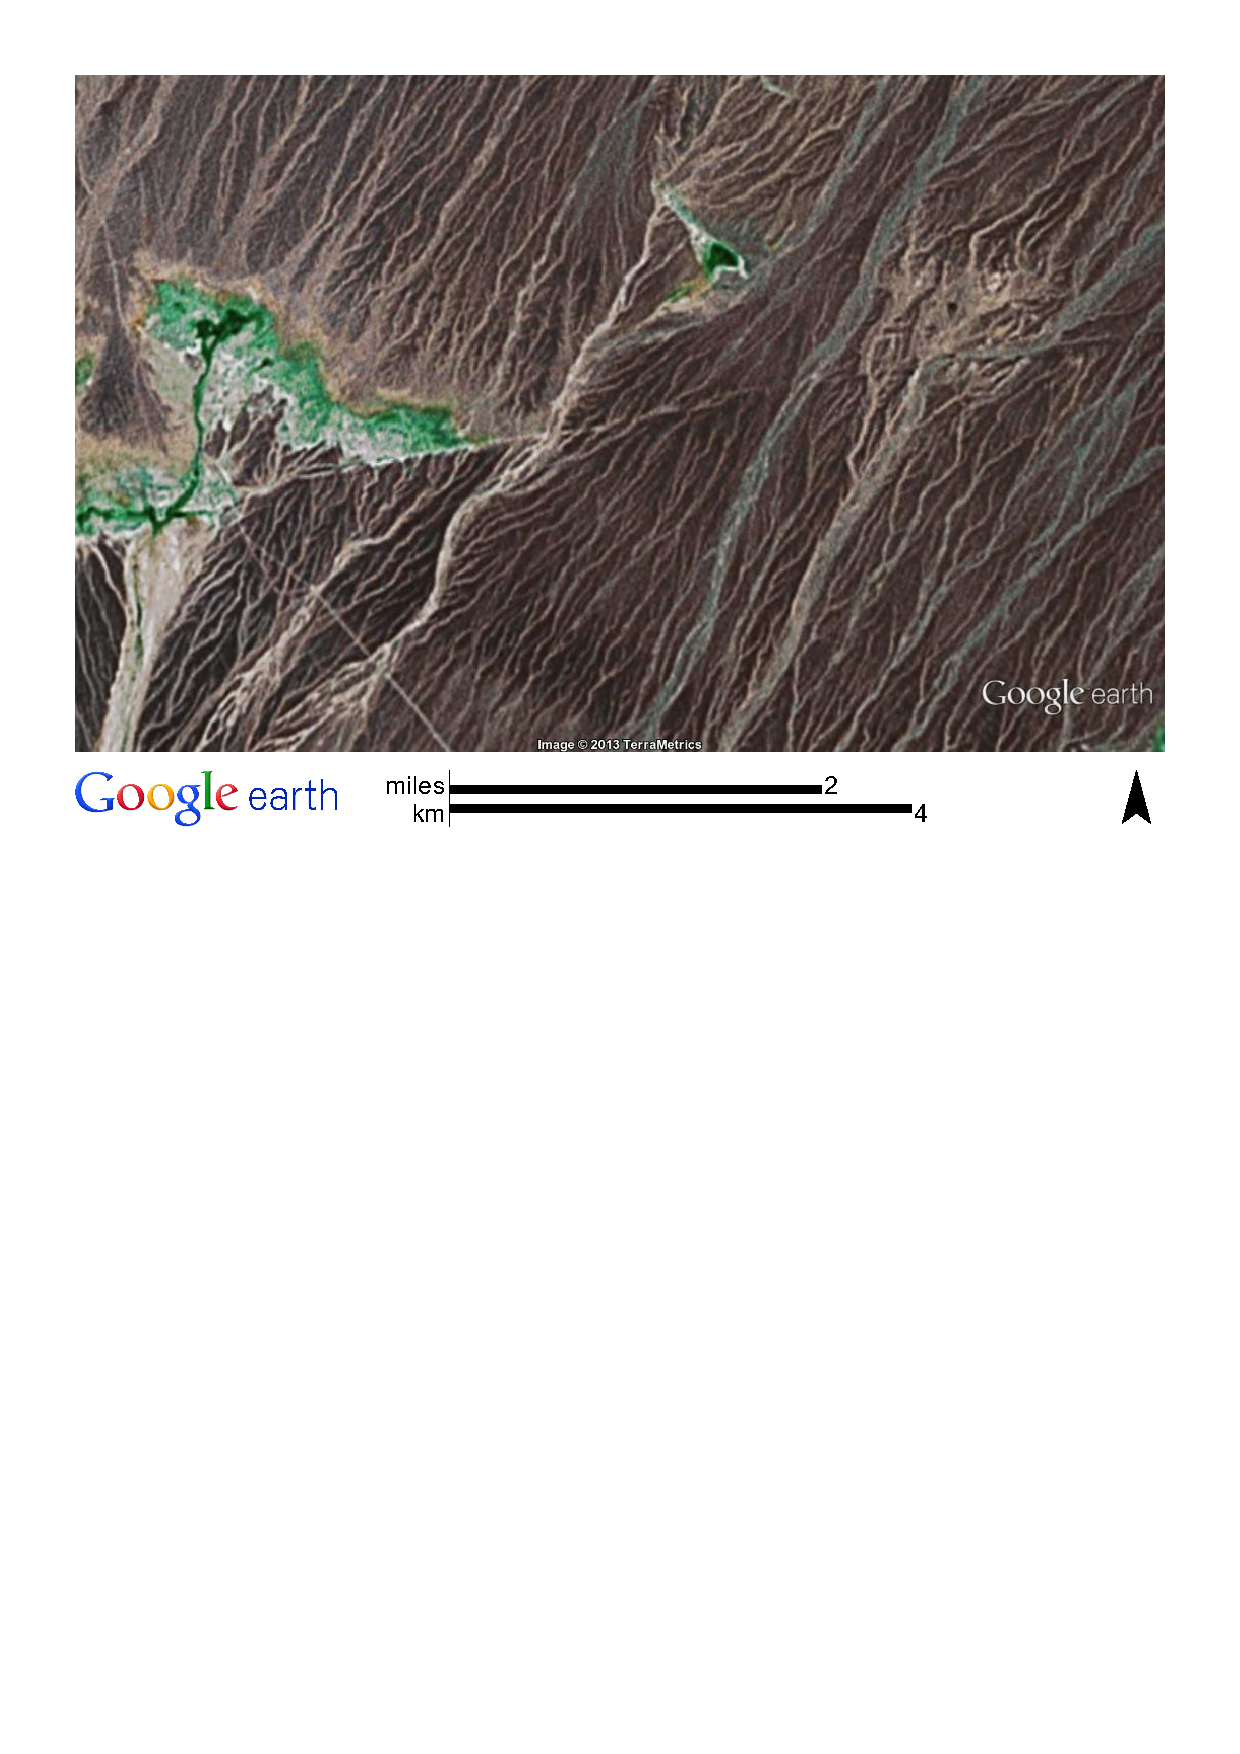
\includegraphics[width = 4in, height = 2.0in]{offsetstreambedsshargyn.png}
  \caption{Offset stream beds along the ENE-WSW striking Shargyn Fault observed in Landsat imagery west of cross-section C-C'.}
  \label{shargynoffsetstreams}
\end{figure}

To the east, the strike of the Shargyn fault bends slightly southwards, at the cross-section marked D-D' in Figure \ref{shargynfaultxsecs}. Here, the fault is still noticeable in satellite imagery (REFERENCE IMAGE). To the south of the fault, we see steep rolling hills with highly deformed and metamorphosed amphibolite and gneiss. To the north of the fault, the topography is lower and transitions into alluvium. The northern unit is an slightly deformed alkali granite (show picture that I took?). Although the granite intrusion is clearly a later event, the contact between the granite and the metamorphic is perfectly straight, supporting the interpretation of a fault. The topographic depression along the fault provides further evidence. To the east, the fault terminates somewhere near the city of Altai. There may be thrust faults that connect the Shargyn Fault with the Khantaishir thrusts, but we did not observe them in the field or on the satellite imagery. 

\subsection{Tonhil Fault and Intersection Wedge Thrusts}
\begin{figure}[h!]
  \centering
  \includegraphics[width = 6in, height = 6.0in]{intersectionwedgexsecs.png}
  \caption{Cross sections through the intersection wedge.}
  \label{intersectionwedgexsecs}
\end{figure}

Further west, the wedge between the Tonhil and Gobi-Altai Faults exhibits some of the most extensive thrusting. 

At the far southern corner of the thrust wedge, we examined the terminus of the Bogd Fault, shown in cross-section J-J' in Figure \ref{intersectionwedgexsecs}. After the various thrust splays further east and north, it is unlikely that there is significant relative motion so far south. However, what remains is directed into a thrust fault that strikes approximately 45 degrees off the main Bogd Fault. There is a noticeable topographic rise bending away form the main Bogd Fault. Though we did not observe the fault itself, the small depositional region and the topographic rise would be unlikely without recent motion. In addition, there was a higher local degree of damage to the bedrock. We observed a fracture set at (FILL IN S/D). 

At the eastern corner of the wedge, there is a bend in the Gobi-Altai Fault from E-W striking to ENE-WSW striking. At the location of this bend, there is a small (2km wide) transtensional basin, shown in cross-section H-H'. This has been previously identified on satellite imagery by authors (CITE THEM!). We examined the area. Though we were not able to directly observe any deformation structures, the southern margin of this basin had a very steep topographic rise. North of the basin, we found a large granite intrusion. South of the basin, there are south (CHECK this in field notebook) dipping high grade metamorphic rocks. Because of the topographic depression and depocenter, the small basin is probably bounded by a normal fault on one side and the left-lateral Bogd Fault on the other. 

The western boundary of the intersection wedge is controlled by the Tonhil Fault. The Tonhil Fault is a major NNW-SSE striking right-lateral strike slip fault. At the cross-section K-K', we examine the fault where it interacts with the northwestern corner of the intersection wedge. At the latitude of the cross-section, the Tonhil fault bends so that it strikes nearly N-S. This bend appears to have created another transtensional basin. We did not examine the transtensional basin in the field. However, it is interesting that it lies symmetrically across the intersection wedge from the transtensional basin on the Bogd Fault examined in cross-section H-H'. 

Further east, along cross-section K-K', we observed a boundary between greenschist grade metasedimentary rocks on the east side and a gneissic unit on the west side. This is interpreted as the furthest northern extent of the southwesternmost of the intersection wedge thrusts. For most of its length, satellite imagery of this fault shows some topographic expression and where observed in the field, it always separates the gneiss and schist from the metasedimentary rocks, indicating that it is an important structural boundary. 

\subsection{Bogd Fault and Termination Thrust Splays}

\begin{figure}[h!]
  \centering
  \includegraphics[width = 6in, height = 3.5in]{bogdfaultxsecs.png}
  \caption{Cross sections through the Shargyn Fault and its termination splays.}
  \label{bogdfaultxsecs}
\end{figure}

Along the southern margin of the basin, we encounter a repeated motif where thrusts splay off the main Gobi-Altai left-lateral strike slip fault. These faults can be seen in the large scale fault map. Two transects were studied across these thrust splays. 

The easternmost of these thrusts can be seen in cross-section F-F' in Figure \ref{bogdfaultxsecs}. Directly above (south) the thrust, there is a complex sequence of metasedimentary and metavolcanic that is intruded by a large gabbro body. A bit to the west of the cross-section line, the topography lowers and outcrop is only visible within a short band near the fault itself. The average strike of the foliation in the fault-adjacent metasedimentary unit is visibly parallel to the fault on satellite imagery. This is confirmed in the field, though minor folding interferes locally. This suggests that the fault follows a pre-existing weakness in the meta-sedimentary unit. Further south along the cross-section, we encounter another fault. The lithology changes sharply from a sandstone and basalt sequence to a greenschist facies metasedimentary sequence. Furthermore, there is another jump in topography at the fault. This fault was never observed. However, the satellite imagery indicates that it dominates the topographic expression west of our fault. 

Twenty five kilometers to the west, we identified and visisted another of these thrust splays at cross-section G-G'. Based on continuous uplift, it appears to be the same fault as the one observed in the southern portion of the Haliun cross-section (F-F'). This fault was visible in outcrop. The fault strikes approximately east and dips 15 degrees. The foot wall consists of low grade metamorphosed mudstones. The hanging wall consists of similar clastic metasedimentary rocks plus greenschist. Inwards, there are multiple layers of brecciated footwall and hanging wall rock and multiple layers of fault gouge. Kinematic indicators suggest thrust sense of motion. A photograph is shown in Figure \ref{faultzones}B. The topography rises sharply directly south of the location of the fault.

\section{Geophysical Data}
	The lack of faulting in the Shargyn Basin is anomalous and could be due to unique basement geology. I derive constraints on the subsurface geology of the Shargyn Basin from geophysical measurements. I examined the available gravity, magnetic and seismic data for the region.

	Bouguer gravity anomaly measurements (shown in Figure \ref{gravity}) indicate that the crust beneath the Shargyn Basin is denser than the surrounding area. Bouguer gravity anomalies are deviations from the geoid gravity field after correcting for the elevation of the measurement and the excess mass above the geoid. A deep crustal root implies lower density and thus, isostasy should cause large elevated regions to show a large negative bouguer anomaly, whereas topographically low regions should show a more positive bouguer anomaly. This can be seen in Figure \ref{gravity}, where the Altai mountain range and the Hangai mountain ranges show very strong negative Bouguer anomalies. The topographically low region south of the Altai and Gobi-Altai and the "Lakes" region, between the Altai and the Hangai both show significantly less negative anomalies, as expected for topographic lows.
	
	Bouguer gravity anomaly measurements were calculated from the EGM2008 global gravity model \citep{EGM2008}, which uses a spherical harmonic expansion through order 2160. Compared to the surrounding mountain ranges, the Shargyn Basin shows a more negative bouguer anomaly. Furthermore, compared to the rest of the region, many of the mountain ranges immediately surrounding the Shargyn Basin show a surprisingly small negative bouguer anomaly. The negative bouguer anomaly beneath the Shargyn Basin can be explained by a denser crustal basement. The small negative bouguer anomaly in the surrounding mountain ranges may indicate lighter than average crustal densities in these regions. \citet{Bayasgalan2005a} calculates an average elastic thickness for Mongolia of ~6km. This elastic thickness would lead to almost complete isostatic adjustment for an area the size of the Shargyn Basin. Hence, the anomaly cannot be attributed to isostatic adjustment from other nearby anomalies, like the Sutai Range. The density anomalies could be linked to the location of past and present faulting. Perhaps, the denser basement under the Shargyn Basin is more difficult to fracture and deform.

\begin{figure}[h!]
  \centering
  \includegraphics[width = 5in, height = 5.0in]{{gravity.ps}.png}
  \caption{Bouguer gravitational anomalies in western Mongolia. The Shargyn Basin is outlined in black. Compare the more negative anomalies under the Shargyn Basin to the more positive anomalies underneath the surrounding mountain ranges. This is the opposite of what we would expect from isostatic considerations.}
  \label{gravity}
\end{figure}

	Magnetic anomalies could also indicate a different composition of crust beneath the Shargyn Basin, however the signal is ambiguous in the Shargyn Basin. I used the NGDC-720 Crustal Magnetic Field Model, a elliptical harmonic expansion of the gravitational field to $n = 720$.  The gravitational anomaly above the Shargyn Basin and surrounding areas is shown in Figure \ref{magnetic}. The Shargyn Basin is at the location of a small positive magnetic anomaly. However, the spatial extent of the anomaly does not match very well with the shape of the Shargyn Basin. This is to be expected, because the minimum resolvable wavelength for a harmonic expansion of order 720 is ~56km. It is also likely that there is significant spatial error near the minimum wavelength. The Shargyn Basin is only 140km across -- less than 3 minimal wavelengths. Therefore, we are currently unable to decide whether there is a real magnetic anomaly beneath the Shargyn Basin. 

\begin{figure}[h!]
  \centering
  \includegraphics[width = 5in, height = 5.0in]{{magnetic.ps}.png}
  \caption{Magnetic anomaly in western Mongolia. The Shargyn Basin is outlined in black. Note the much lower resolution than the gravity measurements.}
  \label{magnetic}
\end{figure}

	Earthquake focal mechanisms provide useful information about active fault slip in the region. The World Stress Map \citep{WorldStressMap2008} uses focal mechanisms as the exclusive constraint on the primary stress axis in western Mongolia due to the lack of other data. \citet{Bayasgalan2005a} provides a good review of the earthquake focal mechanisms in western Mongolia. On the Shargyn Fault, near cross-section C-C', a focal mechanism was calculated showing exclusively left-lateral slip. In the northern corner of the intersection wedge, a focal mechanism was calculated either showing low-angle south directed thrusting or high-angle north directed thrusting. Both possibilities are reasonable given the location of the earthquake. 
		
	Seismic wave speeds underneath the basin could indicate different crustal properties. I investigated available P-wave and S-wave global teleseismic models, but no existing models have sufficient resolution to determine the wave speed anomaly beneath the Shargyn Basin. If there have been local seismological surveys performed, I am unaware of them. 

\section{Formation of the Shargyn Basin}
	It is interesting to ask why the Shargyn Basin exists. The Upper and Lower Khantaishir Thrusts translate a portion of the strike-slip motion north into the Shargyn Fault. Westward (left-lateral) advection of material along the Bogd Fault is transformed into uplift by the Khantaishir thrusts. However, further north, this westward motion continues. The differential motion between this westward motion and the comparatively stationary Shargyn Basin is accomodated on the Shargyn Fault and the Dariv Thrust. But, why does this stepover form at all? Moreover, why did it form in its current position? What does the answer tells us about the tectonic processes at work in the area? These are all fundamentally the same question: what causes a given fault to form in a specific location? This is a deep and difficult question to answer in the general case. However, for the Shargyn Basin, there is a partial answer.

	The first answer to this questions involves pre-existing weaknesses in the crust. Near the stepover, the Bogd Fault bends southward 20-30 degrees. For most of its length, it closely follows the Main Mongolian Lineament. The Main Mongolian Lineament is probably a suture zone and separates a Late Proterozoic and Early Paleozoic orogeny on the north side from a Late Paleozoic orogeny on the south side. The bend in the Bogd Fault may be due to a bend in the Main Mongolian Lineament. Other researchers have mapped the Main Mongolian Lineament as bending southwards in this area. On a broader scale, the Gobi-Altai and Altai ranges both follow the approximate structural grain in Figure \ref{grain}.
	
	In almost all (exluding specific parts of the intersection wedge) of the locations we studied the foliation strikes subparallel to the important fault in the region.  The foliations could be explained by dragging along the fault. With enough slip, regardless of the original foliation is an area, dragging of the foliation near the fault will lead to approximately fault-parallel strike. Dragging can be clearly in the satellite imagery of the beds along the Bogd Fault in the intersection wedge. But, in other locations, such dragging is not visible. The foliations also fit well with a model where faults form along structural weaknesses. Faults forming along weaknesses and dragging probably both contribute to the fault-parallel foliations. 

	The second answer to the question of why the Shargyn Basin formed involves the lithology of the basin basement. Based on the bouguer gravity measurements described, there is a clearly positive density anomaly beneath the Shargyn Basin. Because identifying the exact source of a gravity anomaly is mathematically ill-posed, it is impossible to determine precisely what causes this positive density anomaly. But, it does indicate that something is different. The positive density anomaly combined with the lack of faults cutting the basin suggests a mechanically strong crustal block. The Sichuan and Tarim basins are other, larger, more well-known, examples of mechanically strong crustal blocks. 
	
	The Sichuan basin is underlain by a fast P-wave velocity zone down to 250 km \citep{Royden2008}. A very steep topographic rise surrounds the north and west margins of the topographically low basin. The Sichuan basin is up to 10km deep and ~300km E-W by 200km N-S in extent \citep{Burchfiel2008}. The Tarim basin is much larger. The Tarim basin is thought to be a cratonal block, leading to its strength. The weak Tibetan Plateau is separated from the Tarim Basin by the Altyn Tagh Fault (see Figure \ref{asia}). The northern border of the Tarim Basin is the Tian Shan. The Tian Shan is especially mechanically weak, leading to the concentration of deformation. Both the Sichuan and Tarim basins show very little Mesozoic and Cenozoic deformation compared to their surroundings, indicating that their strength is not a recent development \citep{Neil1997}. The lack of active faults or topography cutting the basins is an obvious indication of their strength. The Junggar, 350km to the southwest of the Shargyn Basin, is also interpreted as a mechanically strong basin, perhaps due to a trapped piece of oceanic crust \citep{Carroll1990a}. 

	As we've discussed, seismic velocity anomalies are too low resolution to determine anything about the Shargyn Basin. But, the Shargyn Basin is surrounded by uplifts, similar to the Tarim or Sichuan Basins. Because of the complex Paleozoic tectonic environment, it is not implausible for a large distinct crustal block to have accreted at the site of the Shargyn Basin. We cannot examine the Shargyn Basin for Paleozoic or Mesozoic deformation, but the largest Paleozoic structure in the area does not intersect the Shargyn Basin. The surface trace of the Main Mongolian Lineament follows the southern boundary of the Shargyn Basin from south of the Khantaishir Range west to the Tonhil Fault. The exact reason for this bend in the Main Mongolian Lineament is unknown, but it could indicate a different past tectonic environment in the Shargyn Basin.

	Notably, we have explained a large basin without any extension. Despite being deeper than most basins in the area (963m above sea level at the deepest), it would unexpected for the Shargyn Basin to have formed by any extensional process. Previous researchers have stated that the region has no normal faulting or transtensional faulting (cite cunningham 2005). The low elevations do not require extension. The "Valley of the Lakes" to the north is at similar elevations. The small transtensional basins near the intersection wedge were the only extensional features we found. However, these transtensional basins are multiple orders of magnitude smaller than the Shargyn Basin. Further to the northeast, there are small normal faults linked by a major strike-slip fault \citep{Walker2006}. These features are also much smaller than the Shargyn Basin. In addition to these arguments, the low elevations could be due to the positive density anomaly. Denser crust would naturally isostatically adjust to be topographically low.

\section{Conclusion}
	The India-Eurasia collision causes deformation through a broad swath of Asia. In central Asia, the Altai Range and Gobi-Altai Range accomodate 10-15\% of the total convergence rate. Hence, western Mongolia has some of the best examples in the world of intracontinental deformation patterns. Here, we studied the zone where the Altai fault system and the Gobi-Altai fault system intersect. Transpressional strike-slip deformation is dominant and results in discrete fault block mountain ranges with small basins in between. The Shargyn Basin is an anomalously large basin for the region and begs explaining. 

	We describe the basin as a combination of two active structures. A left-lateral compressional stepover on the Bogd Fault forms the Khantaishir range and the Shargyn Fault. A conjugate strike-slip intersection between the Bogd Fault and the Tonhil Fault forms a wedge of uplifted material in the southwest corner of the basin. Further uplifts surround the basin due to termination thrust splays from the various strike-slip faults. 

	A density anomaly was identified underneath the Shargyn Basin using bouguer gravity anomaly data. Some difference in crustal basement may explain the density anomaly. Such crustal basement may be mechanically strong and difficult to fault. So, this unique block of crust may be controlling the deformation in the area. The lack of cross-cutting inactive faults indicates that most of the active deformation is occuring on ancient multiply-reactivated faults. Combined with the fact that the Paleozoic and Mesozoic structures in the area steer around the basin, we have further support for a unique crustal block.


\bibliographystyle{plainnat}
\bibliography{/home/tbent/projects/library.bib}

\end{document}
